% This is samplepaper.tex, a sample chapter demonstrating the
% LLNCS macro package for Springer Computer Science proceedings;
% Version 2.21 of 2022/01/12
%

% We import package amsmath before the documentclass to avoid the warning.
% Command '\usepackage{amsmath}' results in the following warning:
% Package amsmath Warning: Unable to redefine math accent \vec.
\RequirePackage{amsmath} % for environments such as align

\documentclass[runningheads]{llncs}
%
\usepackage[T1]{fontenc}
% T1 fonts will be used to generate the final print and online PDFs,
% so please use T1 fonts in your manuscript whenever possible.
% Other font encondings may result in incorrect characters.
%
\usepackage{graphicx}
% Used for displaying a sample figure. If possible, figure files should
% be included in EPS format.
%
% If you use the hyperref package, please uncomment the following two lines
% to display URLs in blue roman font according to Springer's eBook style:
%\usepackage{color}
%\renewcommand\UrlFont{\color{blue}\rmfamily}
%


\usepackage{amssymb} % for \mathbb
\usepackage{cleveref} % for \cref
\usepackage{bbm} % for \mathbbm
\usepackage{booktabs} % for \toprule, \midrule, \bottomrule
\usepackage{pgffor} % for \foreach
\usepackage{csvsimple} % for \csvreader
\usepackage{array} % for m column type

% Fig. 1a -> Fig. 1(a)
\usepackage[labelformat=simple]{subcaption}
\graphicspath{{./data/}{./python/data/}}
\renewcommand\thesubfigure{(\alph{subfigure})}
\makeatletter
\def\caption@documentclass{elsarticle}%
\makeatother


\usepackage{algorithm}
\usepackage{algpseudocode}

\newcommand{\ispace}{\mathbb{D}^{m}}
\newcommand{\Prec}{\operatorname{acc}}
\newcommand{\Cov}{\operatorname{cov}}
\newcommand{\cands}{\bar{\mathcal{A}}}
\algnewcommand{\IIf}[1]{\State\algorithmicif\ #1\ \algorithmicthen\ }
\renewcommand{\algorithmicrequire}{\textbf{Input:}}
\renewcommand{\algorithmicensure}{\textbf{Output:}}


\begin{document}
%
\title{%
  R-LIME: Rectangular Constraints and Optimization for Local Interpretable
  Model-agnostic Explanation Methods}
%
\titlerunning{%
  R-LIME: Rectangular Constraints and Optimization for LIME Methods
}
% If the paper title is too long for the running head, you can set
% an abbreviated paper title here
%
\author{Genji Ohara\inst{1}\orcidID{0009-0000-5854-2820} \and
  Keigo Kimura\inst{1}\orcidID{0000-0002-3614-6568} \and
  Mineichi Kudo\inst{1}\orcidID{0000-0003-1013-3870}
}
%
\authorrunning{G. Ohara et al.}
% First names are abbreviated in the running head.
% If there are more than two authors, 'et al.' is used.
%
\institute{Division of Computer Science and Information Technology\\
  Graduate School of Information Sci.\ and Tech.,
  Hokkaido University\\
  Sapporo 060-0814, JAPAN,\\
  \email{\{genji-ohara, kimura5, mine\}@ist.hokudai.ac.jp}}

\maketitle              % typeset the header of the contribution
%
% The abstract should briefly summarize the contents of the paper in
% 150--250 words.

\begin{abstract}
  In recent years, complex machine learning models such as deep neural networks
  have been used in various industrial fields due to their high accuracy.
  However, its complexity has been a major obstacle to implementation
  in decision-making situations where transparency of the decision process is required.
  In order to solve this problem,
  various post-hoc explanation methods have been proposed,
  but they have not been able to achieve interpretability of
  both the explanation and its scope.
  We propose a new method that interprets complex models in an interpretable
  approximation region.
  R-LIME locally approximizes a complex decision boundary with a linear classifier
  and maximizes the approximation region as long as the accuracy of the linear
  model is higher than a specified threshold.
  We demonstrate the effectiveness of the proposed method through a qualitative
  and quantitative evaluation using a real-world dataset.
  Finally, we discuss limitations and future work of the proposed method.
  % 148 words
  \keywords{Interpretable machine learning \and Local surrogate model}
\end{abstract}

\section{Introduction}
Machine learning models, such as deep learning and random forests,
have been widely employed in various industrial applications
due to their significant improvement in accuracy in recent years.
However,
the increasing complexity and black-box nature of these models pose challenges,
particularly in critical decision-making scenarios like healthcare and finance,
where the opacity of decision rationale becomes a major obstacle to 
implementation.
Consequently,
there has been extensive research in the field of post hoc explanation
for machine learning models \cite{%
  ribeiro2016why,ribeiro2018anchors,radulovic2023bella,guidotti2018local}.

Existing studies on post hoc explanations categorize into model-dependent and
model-agnostic methods,
depending on their dependence on the model's structure.
Model-dependent methods primarily focus on deep neural networks and
explain the model's behavior using internal parameters.
While they allow a direct approach to the model, 
applying the same method to models with different structures is often challenging. On the other hand, model-agnostic methods do not rely on internal parameters and utilize only the model's output. Although they provide high generality, their information is constrained, making them more versatile. Model-agnostic methods further classify into global and local methods based on their treatment of input space. Global methods aim to explain the model's behavior across the entire input space, seeking explanations valid for any input. However, providing global explanations becomes challenging as the model's complexity increases. Local methods, in contrast, explain the model's output for a specific input (focus point) in the vicinity of that input. While local methods offer simple and accurate explanations compared to global methods, their applicability is limited.

This paper specifically focuses on model-agnostic and local methods. For instance, Local Interpretable Model-agnostic Explanations (LIME) \cite{ribeiro2016why} approximates the complex model's decision boundary locally using a simpler model. Although LIME enables users to interpret the local behavior of complex models, it has been criticized for not optimizing the approximation region \cite{radulovic2023bella} and not presenting the approximation region in an interpretable form \cite{ribeiro2018anchors}.

To address the limitations of LIME,
we propose an algorithm that interprets complex models
in an interpretable approximation region,
taking inspiration from another explanation method called Anchor
\cite{ribeiro2018anchors}.
Our proposed method maximizes the accuracy of the learned approximation model
within a rectangular approximation region under lower-bound constraints.
The resulting rectangular region is expressed as a conjunction of predicates
related to features, enhancing interpretability for the user.

\section{Related Work}
The figures presented visually compare three methods: LIME, Anchor, and BELLA.

\begin{figure}[t]
  \vspace{0.5cm}
  \begin{subfigure}[t]{\textwidth}
    \centering
    
\includegraphics[width=0.55\textwidth]{lime_vs_anchor_exp_a.png}
    \caption{Instance around the focal point.}\label{fig:lime_vs_anchor_exp_a}
    \vspace{0.5cm}
  \end{subfigure}
  \hfill
  \begin{subfigure}[t]{\textwidth}
    \centering
    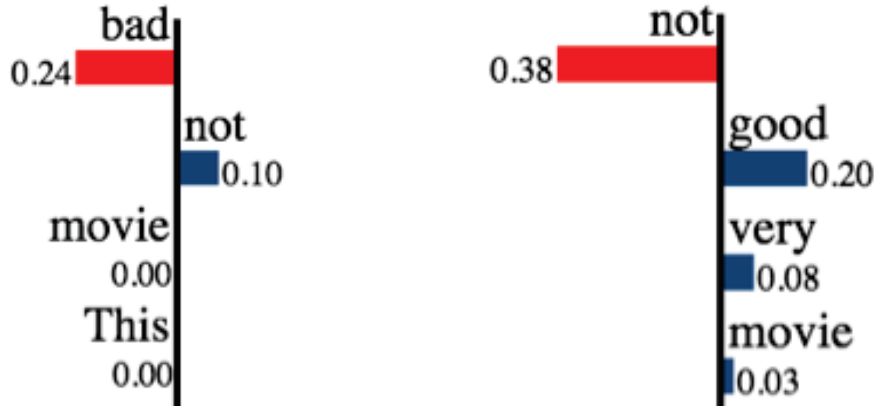
\includegraphics[width=0.4\textwidth]{lime_vs_anchor_exp_b.png}
    \caption{Explanation by LIME.}\label{fig:lime_vs_anchor_exp_b}
    \vspace{0.5cm}
  \end{subfigure}
  \begin{subfigure}[t]{\textwidth}
    \centering
    
\includegraphics[width=0.55\textwidth]{lime_vs_anchor_exp_c.png}
    \caption{Explanation by Anchor.}\label{fig:lime_vs_anchor_exp_c}
  \end{subfigure}
  \caption[Examples of output results by LIME and Anchor]{Examples of output results by LIME and Anchor \cite{ribeiro2018anchors}.}\label{fig:lime_vs_anchor_exp}
\end{figure}
In this chapter, we provide an overview of existing research on model-agnostic and local post hoc explanations, particularly focusing on studies closely related to the proposed method.

\subsection{LIME (Local Interpretable Model-agnostic Explanations) \cite{ribeiro2016why}}
LIME is a method for locally approximating a trained black-box classifier $f: \mathbb{R}^d \to \{0,1\}$ around a focal point $x \in \mathbb{R}^d$ using a linear model $g: \mathbb{R}^d \to \{0,1\}$ (\cref{fig:lime}). The process involves:
\begin{enumerate}
  \item Obtaining a set of perturbed samples $\mathcal{Z}_p$ around $x$ and the set of pseudo-labels $f(\mathcal{Z}_p) = \{f(z) \mid z \in \mathcal{Z}_p\}$.
  \item Learning an interpretable model $g$ using $\mathcal{Z}_p$ and $f(\mathcal{Z}_p)$ by minimizing the following loss function:
        \begin{equation}
          \label{eq:lime_loss}
          \mathcal{L}(f,g,\pi_x)=\sum_{z\in\mathcal{Z}_p}
          \pi_x(z){\left(f(z)-g(z)\right)}^2,
        \end{equation}
        where $\pi_x(z)$ is a weight function designed to be larger for samples closer to $x$, typically implemented using an exponential kernel.
\end{enumerate}

LIME provides valuable insights into the local behavior of the model by showing the contribution of each feature to the output $f(x)$. However, due to not explicitly indicating the perturbation region, users cannot assess the effective scope of the explanation \cite{ribeiro2018anchors}. An example explanation for an LSTM sentiment prediction model using LIME is illustrated in \cref{fig:lime_vs_anchor_exp_b}. The left explanation suggests that the word "not" contributes to the model's positive prediction, which does not apply to the instance on the right. However, without the explicit perturbation region, users might mistakenly apply the left explanation to the right instance, potentially leading to a misunderstanding of the black-box model's behavior \cite{ribeiro2018anchors}.

\subsection{Anchor \cite{ribeiro2018anchors}}\label{sec:anchor}
Anchor represents a rectangular region, expressed as a conjunction of predicates (rules) related to features, that maximizes the probability of the black-box classifier $f$ outputting $f(x)$ within the region. It aims to highlight important features contributing significantly to the output (\cref{fig:anchor}).

For a discrete $m$-dimensional input space $\ispace$ with a trained black-box classifier $f: \ispace \to \{0,1\}$, an instance $x \in \ispace$, and a distribution $\mathcal{D}$ over the input space, a rule $A(z) = a_{i_1}(z) \wedge a_{i_2}(z) \wedge \dots \wedge a_{i_t}(z)$ is defined. The predicates $a_i(z)$ evaluate to true ($=1$) when $z_i = x_i$ and false ($=0$) otherwise. The precision $\Prec(A)$ and coverage $\Cov(A)$ of the rule $A$ are defined as follows:
\begin{align}
  \Prec(A) & =\mathbb{E}_{z\sim\mathcal{D}(z|A)}
  [\mathbbm{1}_{f(z)=f(x)}], \label{eq:anchor_def_prec} \\
  \Cov(A)  & =\mathbb{E}_{z\sim\mathcal{D}(z)}[A(z)].
\end{align}

Here, $\mathcal{D}(z|A)$ is the conditional distribution in the region where the rule $A$ is true.
% When sampling the perturbation vector $z$ according to the distribution $\mathcal{D}$,
$\Prec(A)$ represents the probability that the output of $f$ matches between the perturbation $z$ and the focal point $x$ in the region $A$, and $\Cov(A)$ expresses the probability that the perturbation $z$ fits into $A$.

An Anchor maximizes coverage within the given threshold $\tau$ while maintaining precision.
However, direct computation of \cref{eq:anchor_def_prec} is not feasible, and it is evaluated using PAC (Probably Approximately Correct) through sampling.
Introducing a confidence level $1-\delta$ $(0\le\delta\le1)$, the precision constraint is relaxed as follows:
\begin{equation}
  \label{eq:const_prec}
  P(\Prec(A)\ge\tau)\ge1-\delta.
\end{equation}
Thus, the following optimization problem is solved:
\begin{equation}
  \label{eq:main_problem}
  A^*=\underset{A \text{ s.t. } P(\Prec(A)\ge\tau)\ge1-\delta\wedge A(x)=1}
  {\arg\max}\Cov(A).
\end{equation}

While Anchor provides a clear presentation of the effective scope of the explanation, the information it includes is less than LIME, limiting its utility \cite{ribeiro2018anchors}. An example explanation for an LSTM sentiment prediction model using Anchor is depicted in \cref{fig:lime_vs_anchor_exp_c}. The left explanation suggests that changing words other than "not" and "bad" has little impact on the classifier's output. While it clearly does not apply to the right instance, the explanation does not provide details about the influence of words like "not" or "bad," resulting in less user insight into the model's behavior compared to LIME (\cref{fig:lime_vs_anchor_exp_b}).

\subsection{BELLA (Black box model Explanations by Local Linear Approximations) \cite{radulovic2023bella}}
BELLA addresses the non-optimization of the approximation region, a drawback of LIME, by learning a local linear approximation model $g$ using a subset $Z'$ of the dataset $Z$ instead of perturbed samples (\cref{fig:bella}). The process involves:
\begin{enumerate}
  \item Computing the distance $d_x(z)$ for all instances $z$ in $Z$ with respect to the focal point $x$.
  \item Selecting the $k$ instances with the smallest $d_x(z)$, forming a subset $Z_s(k) \subseteq Z$.
  \item Learning the local linear approximation model $g$ using $Z_s(k)$ and calculating the similarity measure $\mathcal{R}(k)$ between $f$ and $g$.
  \item Obtaining the optimal $k^*$ by maximizing $\mathcal{R}(k)$.
\end{enumerate}

BELLA aims to enhance the reliability of explanations by optimizing the approximation region for high-accuracy linear approximations. However, it assumes direct access to the dataset $Z$ used for training the classifier, making it inapplicable in scenarios where direct access to the dataset is restricted for privacy reasons. Additionally, as BELLA presents the approximation region as a subset of the dataset, its interpretability is lower compared to Anchor.

\section{Proposed Method}
\begin{figure}[tb]
  \centering
  \begin{subfigure}[t]{0.45\textwidth}
    \centering
    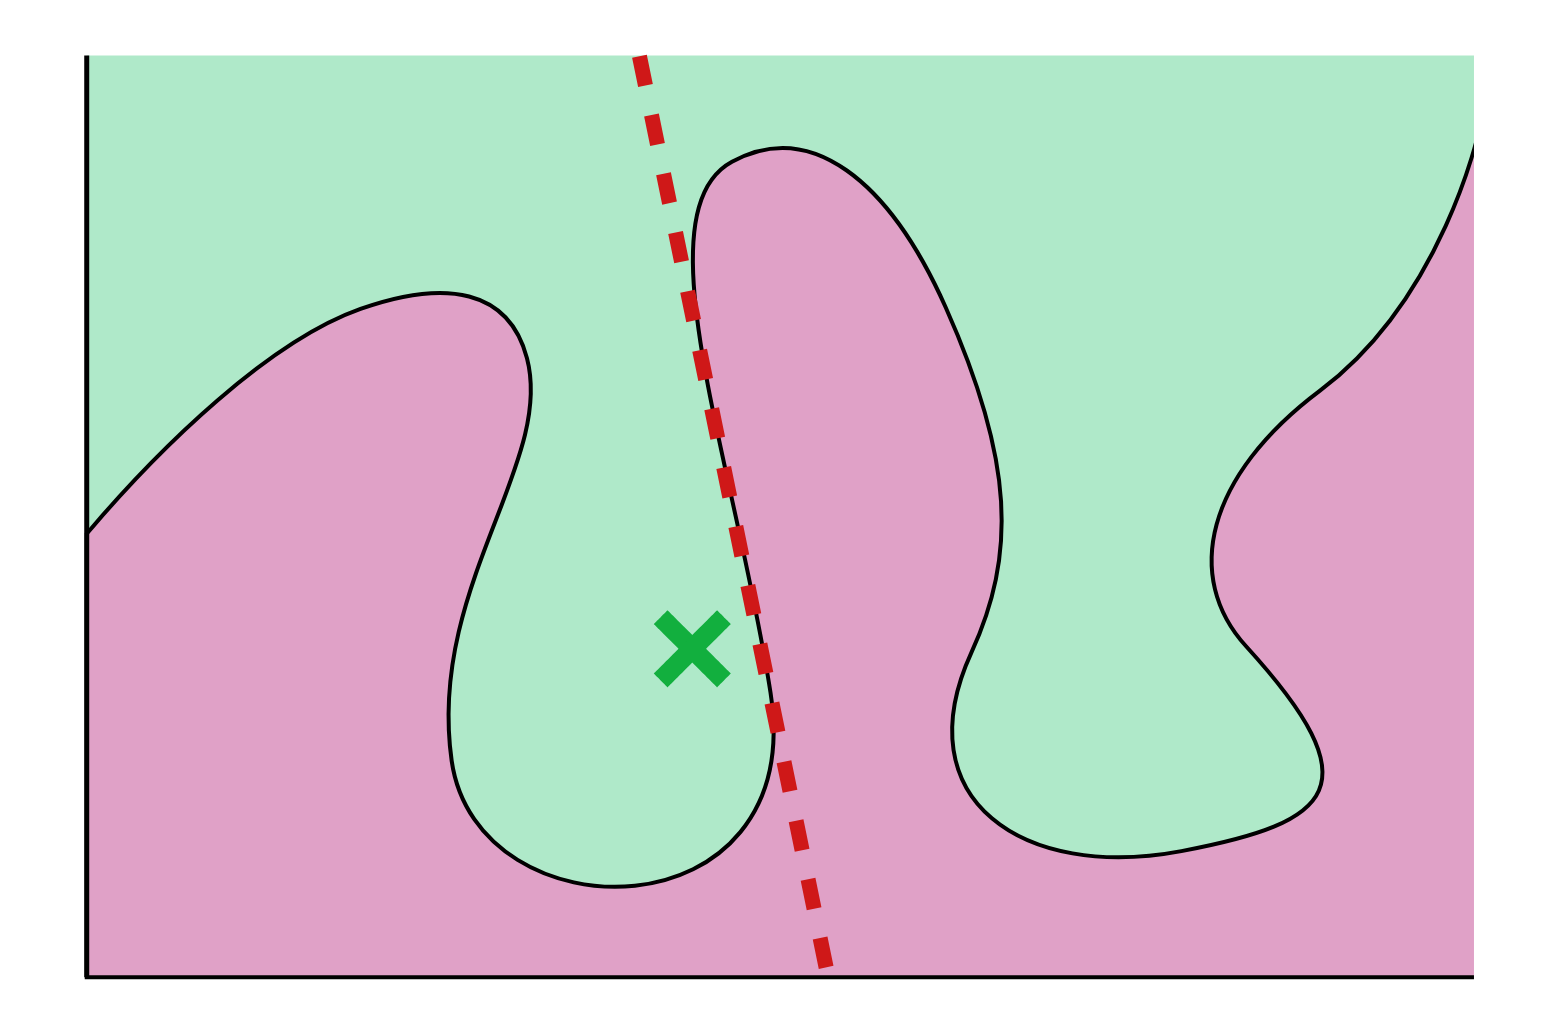
\includegraphics[width=\textwidth]{lime}
    \caption{%
      LIME: Locally approximates decision boundaries around the focal point.}\label{fig:lime}
  \end{subfigure}%
  \hfill
  \begin{subfigure}[t]{0.45\textwidth}
    \centering
    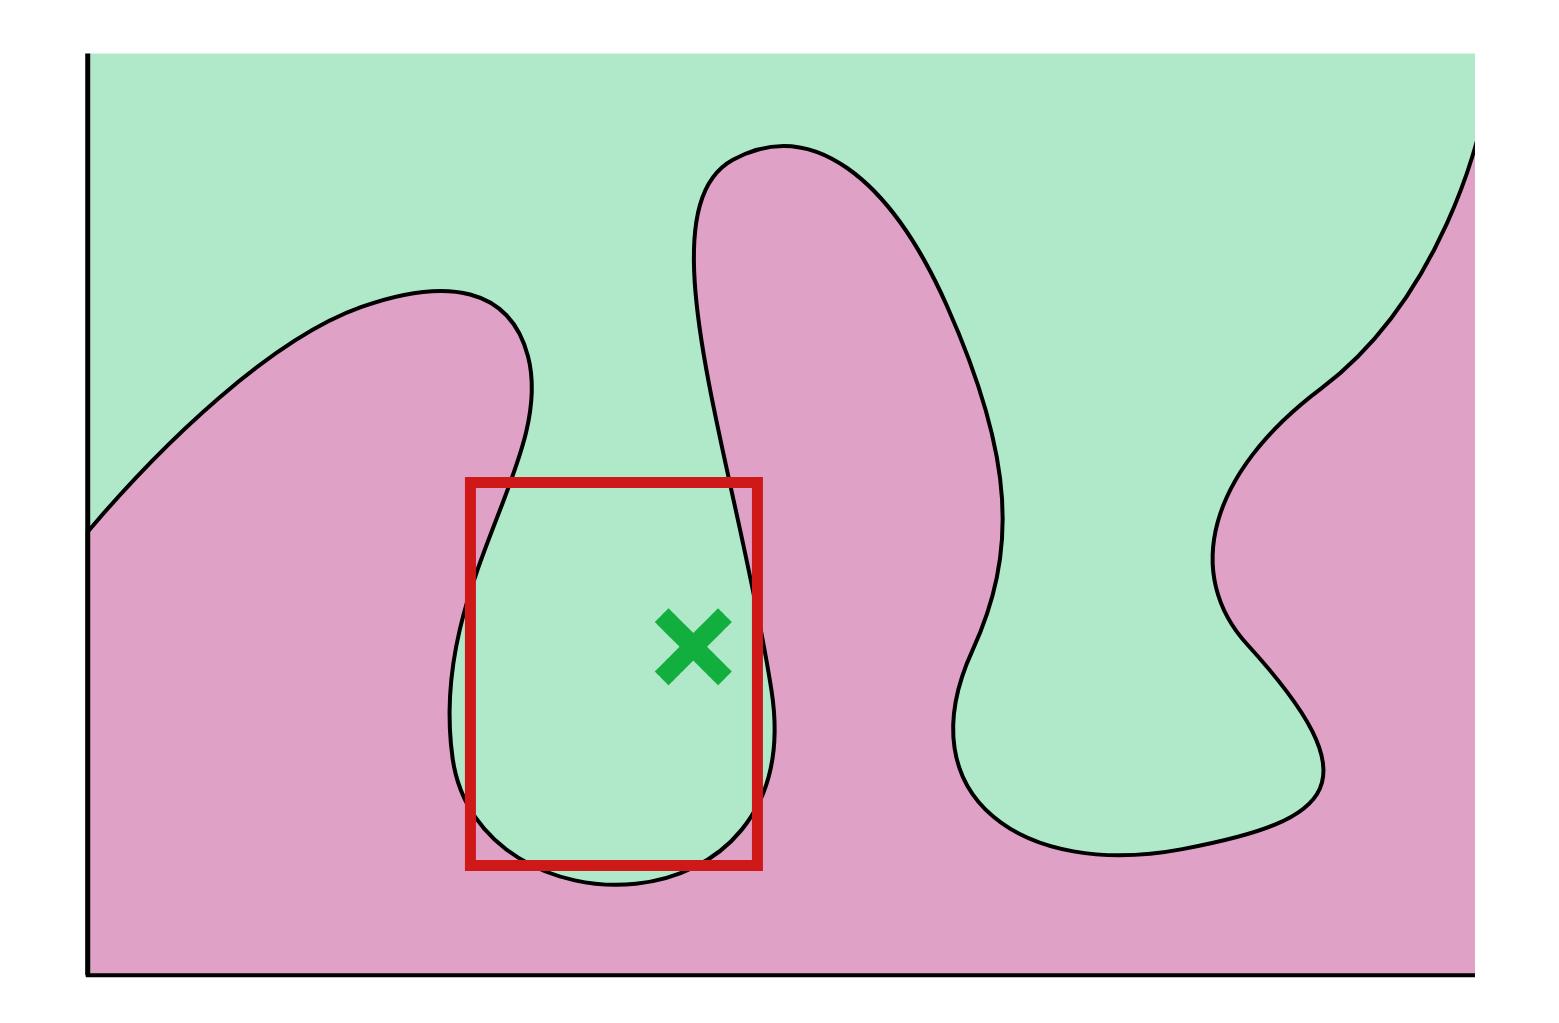
\includegraphics[width=\textwidth]{anchor}
    \caption{Anchor: Maximizes coverage of a rectangular region containing the focal point under precision constraints.}\label{fig:anchor}
  \end{subfigure}
  \hfill
  \begin{subfigure}[t]{0.45\textwidth}
    \centering
    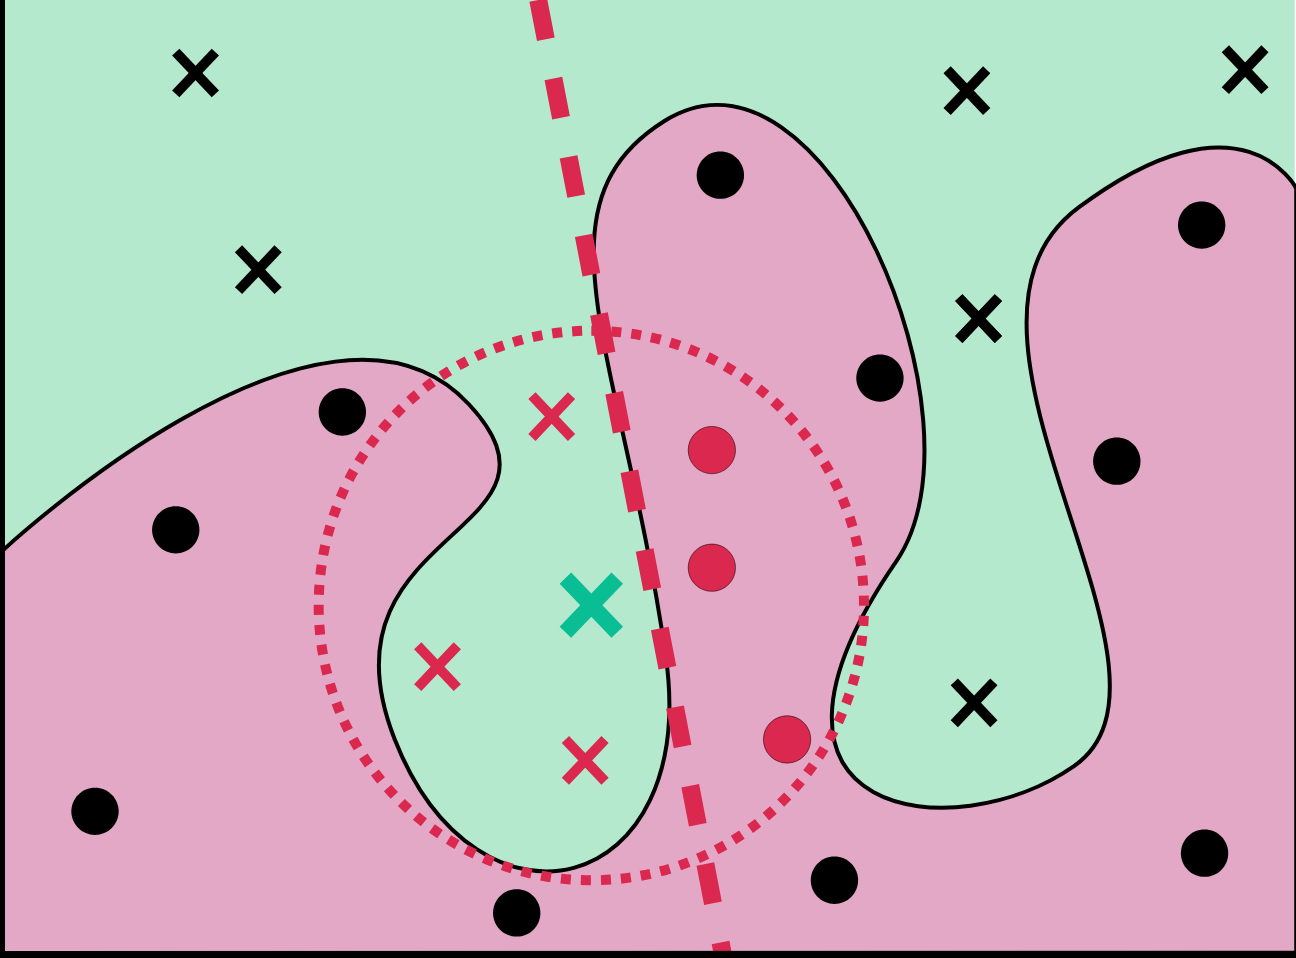
\includegraphics[width=0.85\textwidth]{bella}
    \caption{%
      BELLA: Explores a subset of the dataset, maximizing similarity between the local linear approximation model and the black-box classifier.}\label{fig:bella}
  \end{subfigure}
  \hfill
  \begin{subfigure}[t]{0.45\textwidth}
    \centering
    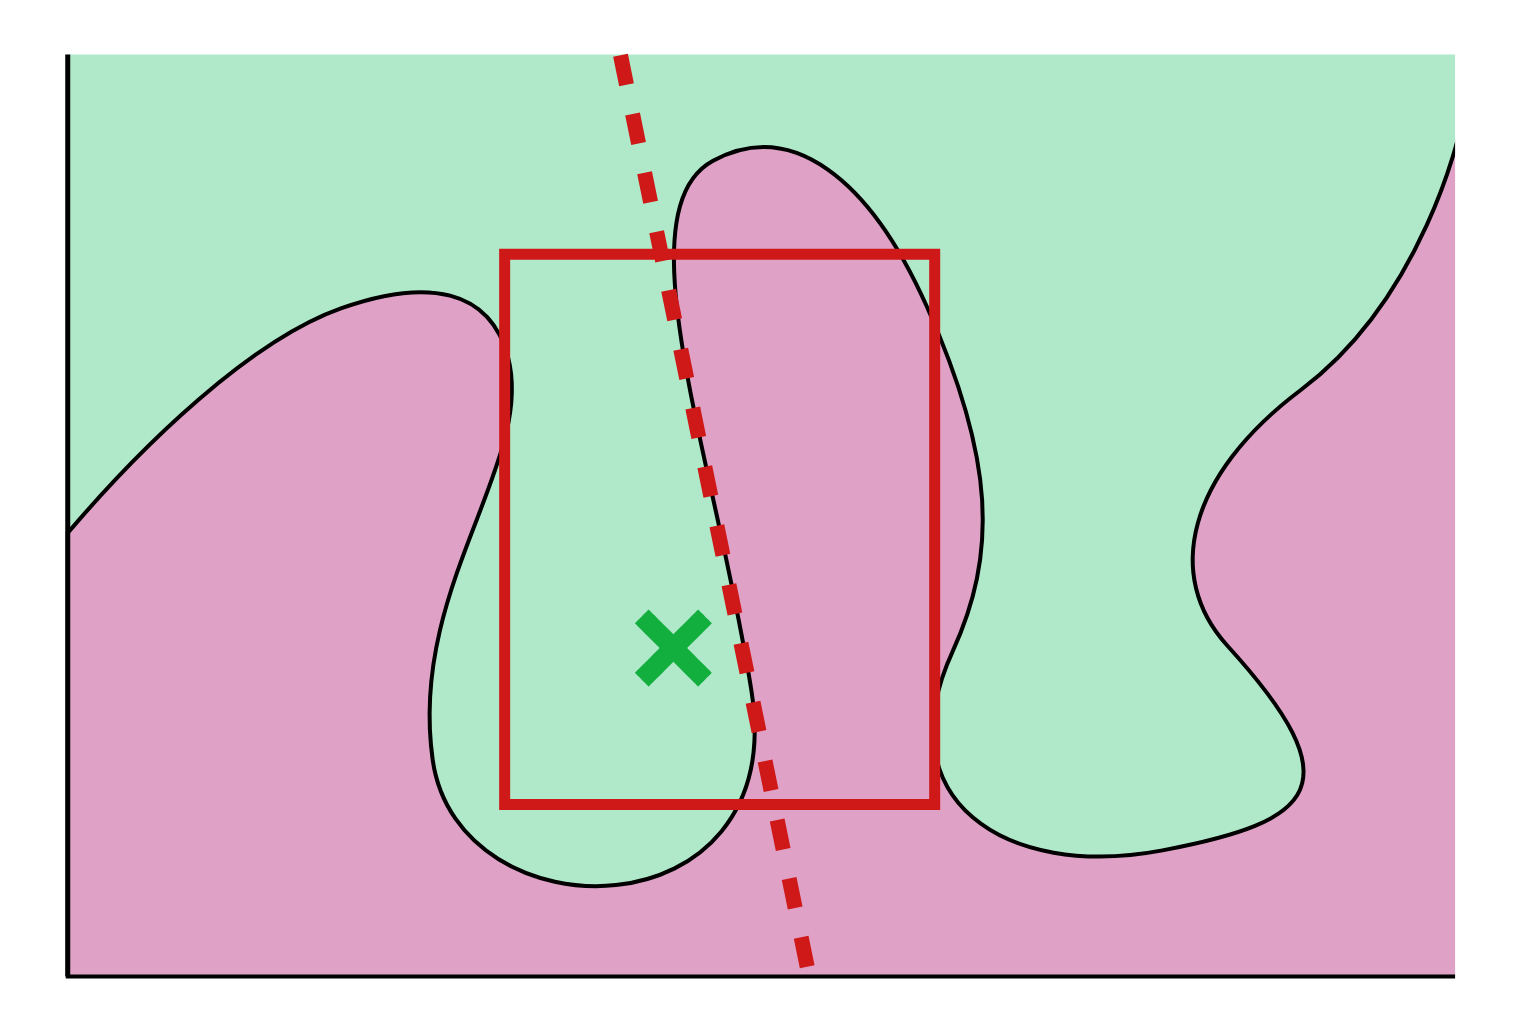
\includegraphics[width=\textwidth]{rlime3}
    \caption{%
      R-LIME: Maximizes coverage of a rectangular region containing the focal point under lower constraints on the accuracy of the approximation model.}\label{fig:rlime}
  \end{subfigure}
  \caption{%
    Visual comparison of LIME, Anchor, BELLA and R-LIME (our proposed method).
    The solid line represents the rectangular region containing the focal
    point, and the dashed line represents the learned approximation model.
  }
\end{figure}

\subsection{Overview}
The proposed method aims to overcome the limitations of LIME \cite{ribeiro2016why} and its improvement methods such as Anchor \cite{ribeiro2018anchors} and BELLA \cite{radulovic2023bella}. Similar to LIME, the proposed method locally approximates the given black-box classifier $f$ around the focal point $x$ using a linear model $g$. However, by adopting a rectangular perturbation region similar to Anchor, it represents predicates (rules) concerning features. The accuracy of explanations is defined as the "accuracy" of rules, and the "coverage" of rules defines the generality of explanations. The proposed method maximizes coverage under lower constraints on accuracy (\cref{fig:rlime}).

Anchor maximizes the coverage of region $A$ within which the output of the black-box classifier $f$ matches $f(x)$ with respect to the probability under lower constraints. The proposed method, on the other hand, learns an approximation model $g$ within the rectangular region $A$ and maximizes the coverage of $A$ under lower constraints on the accuracy of $g$. We modify the definition of accuracy using \cref{eq:anchor_def_prec} as follows:
\begin{equation}
  \Prec(A)=\underset{g\in G}{\max}\ \mathbb{E}_{z\sim\mathcal{D}(z|A)}
  [\mathbbm{1}_{f(z)=g(z)}]. \label{eq:def_prec}
\end{equation}
Here, $G$ represents the set of possible linear approximation models. By solving the optimization problem in \cref{eq:main_problem} under this modified accuracy definition, we can select rules that learn high-accuracy approximation models, among which the coverage is maximized. The proposed method's algorithm, shown in \cref{sec:alg}, is largely based on the algorithms used in Anchor.

In this paper, we refer to the proposed method as "R-LIME" (Ruled LIME). The characteristics of R-LIME are listed below:
\begin{itemize}
  \item The perturbation vector's generation region is optimized and presented in a user-interpretable format.
  \item Interpretation is conducted without direct access to the dataset, utilizing only the distribution.
  \item The number of samples is dynamically determined based on the estimated accuracy without the need for a predefined amount.
\end{itemize}
% This enables model interpretation without direct access to the data, even in scenarios with significant privacy constraints. The optimized and presented explanation's applicable range allows users to evaluate the reliability and generality of the generated explanations.

\subsection{Algorithm}\label{sec:alg}
{%
  \begin{figure}[t]
    \centering
    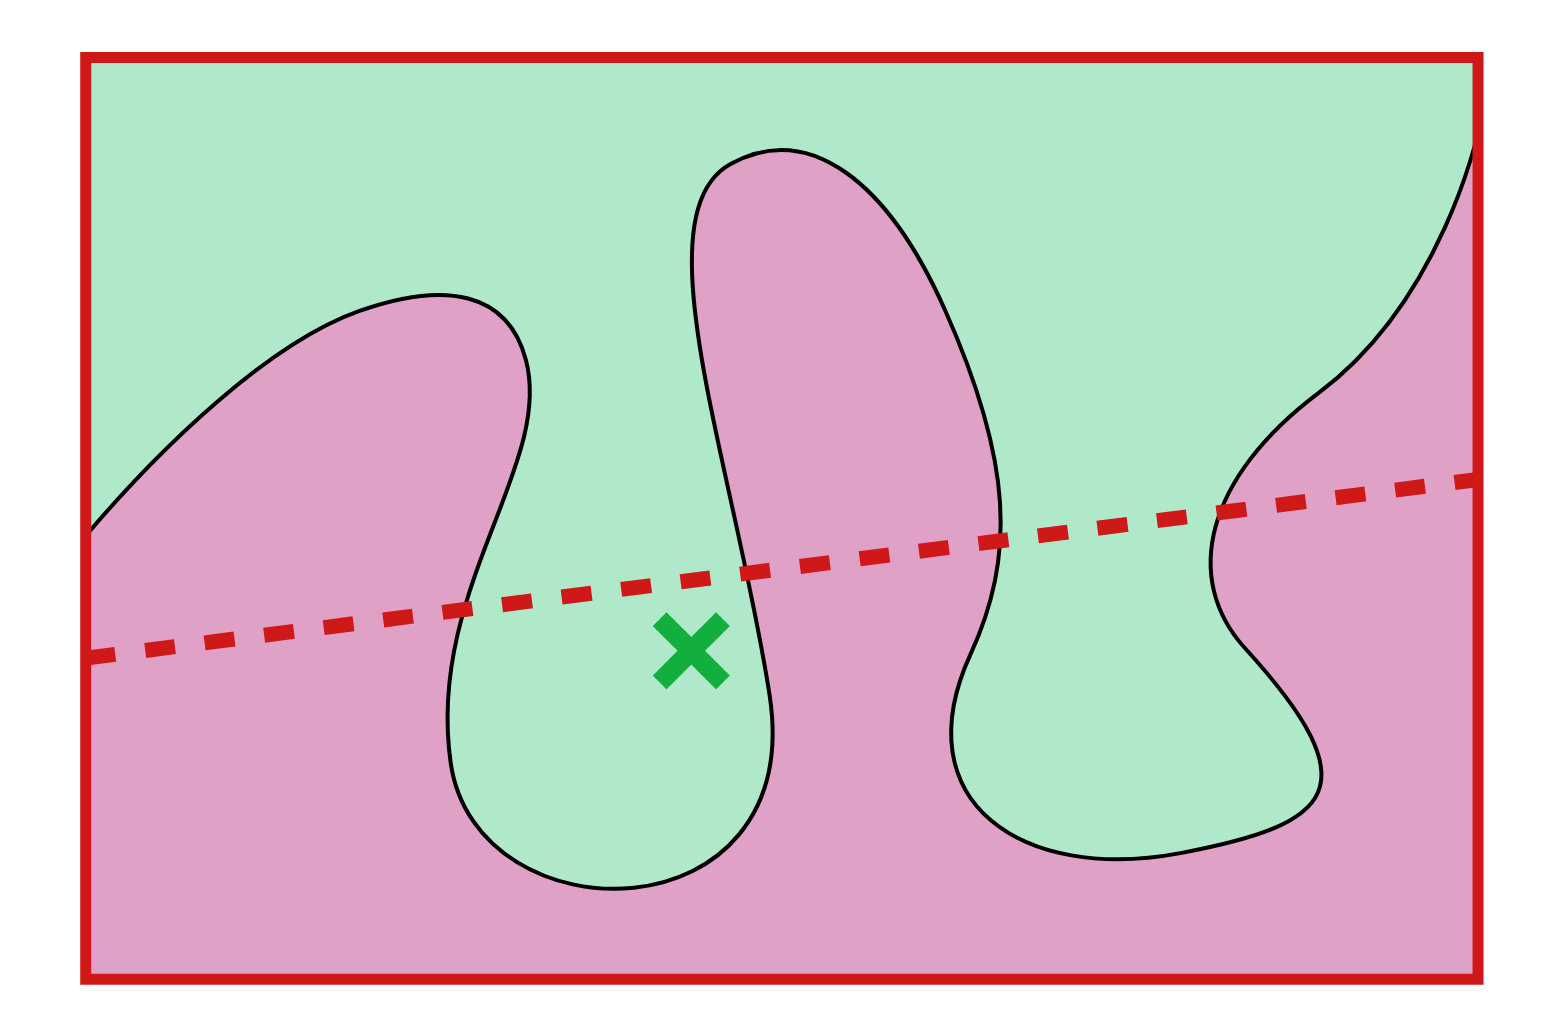
\includegraphics[width=0.32\textwidth]{rlime1}
    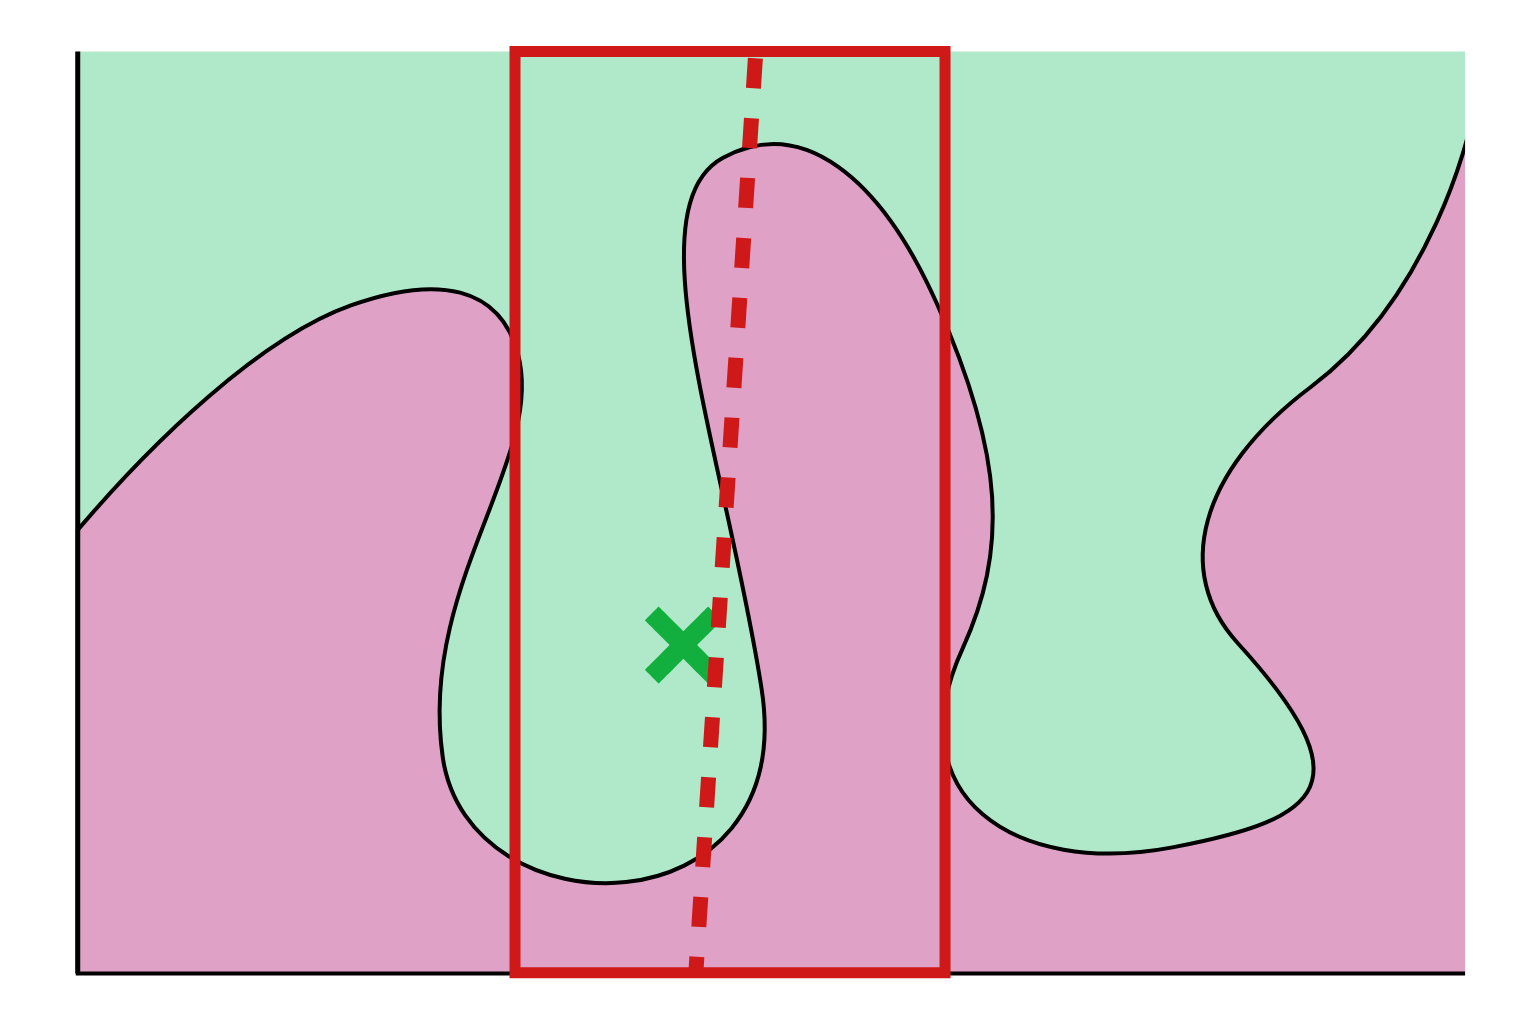
\includegraphics[width=0.32\textwidth]{rlime2}
    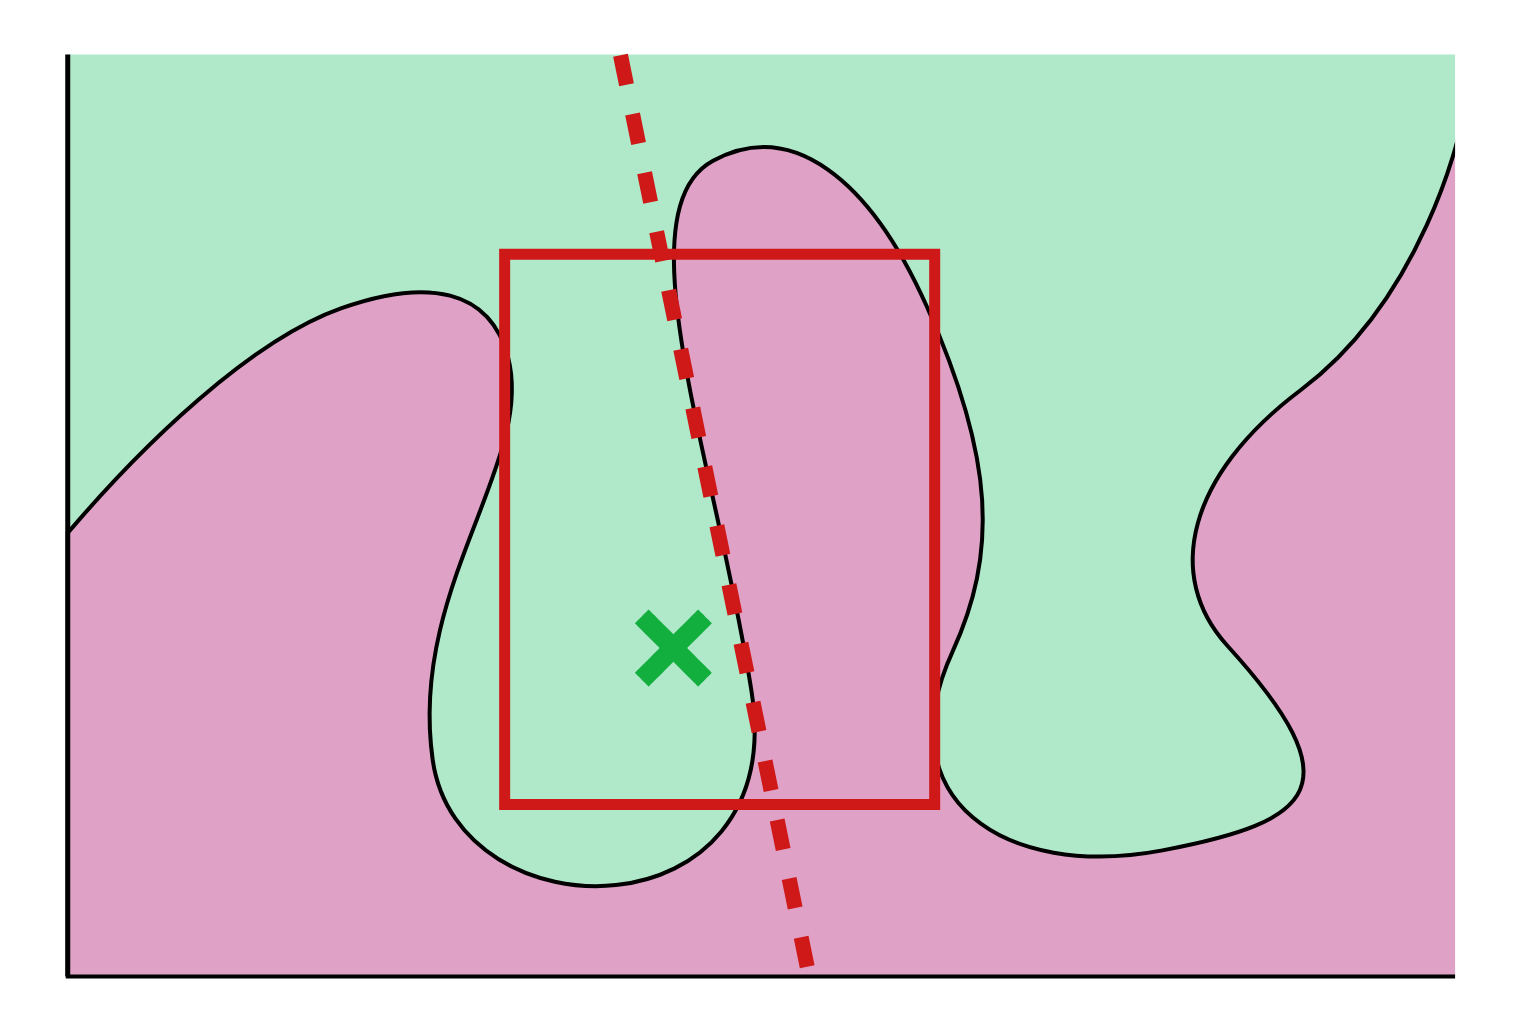
\includegraphics[width=0.32\textwidth]{rlime3}
    \caption[Overview of the R-LIME Algorithm]{%
      Overview of the R-LIME algorithm. The progression of the algorithm from left to right is illustrated. The solid red line represents the rectangular region $A$, and the red dashed line represents the linear approximation model $g$ learned within $A$. The initial value of $A$ is an empty rule (entire input space), and predicates are added to $A$, reducing coverage. The process continues until $\Prec(A)\ge\tau$, at which point the rule with the maximum coverage is output.
    }
  \end{figure}
  \begin{algorithm}[p]
    \caption{R-LIME}\label{alg:greedy-search}
\begin{algorithmic}[1]
	\Require{%
		Black-box model $f$, Target instance $x$,
		Distribution $\mathcal{D}$,
		Threshold $\tau$, Beam width $B$, Tolerance $\epsilon$,
		Confidence level $1-\delta$
	}
	\Ensure{%
		Rule $A^*$ satisfying Eq.~\eqref{eq:main-problem}
	}
	\State{$A^*\gets\textbf{null},\ \mathcal{A}_0\gets\emptyset,\ t\gets0$}
	% \Comment{%
	%   Initialize the set of candidate rules $\mathcal{A}_0$ to $\emptyset$
	% }
	\Comment{Initialize the set of candidate rules $\mathcal{A}_0$ to $\emptyset$}
	\While{$A^*=\textbf{null}$}
	\State$t\gets t+1$
	\State$\cands_t\gets$ \Call{GenerateCands}
	{$\mathcal{A}_{t-1}$}
	\State$\mathcal{A}_t\gets$ \Call{B-BestCands}
	{$\cands_{t},\mathcal{D},B,\epsilon,\delta$}
	\State$A^*\gets$ \Call{LargestCand}
	{$\mathcal{A}_t,\tau,\delta$}
	\EndWhile%
\end{algorithmic}

  \end{algorithm}
  \begin{algorithm}[p]
    \caption{Generating new candidate rules}\label{alg:generate-cands}
\begin{algorithmic}[1]
	\Function{GenerateCands}{$\mathcal{A},x$}
	\IIf{$\mathcal{A}=\emptyset$}{\Return{$\{\mathit{true}\}$}}
	\Comment{An initial empty rule always returns $\mathit{true}$}
	\State$\cands\gets\emptyset$
	\ForAll{$A\in\mathcal{A}$}
	\ForAll{$a\in (T(x)\setminus A)$}
	\State$\cands\gets\bar{\mathcal{A}}\cup(A\wedge a)$
	\Comment{Get a new rule by adding a new predicate $a$ to $A$}
	\EndFor%
	\EndFor%
	\State\Return{$\cands$}
	\EndFunction%
\end{algorithmic}

  \end{algorithm}
  \def\myidt{\hspace{\algorithmicindent}}
  \begin{algorithm}[p]
    \caption{%
	Searching rules with highest accuracy (KL-LUCB~\cite{kaufmann2013information})
}\label{alg:best-cands}
\begin{algorithmic}[1]
	\Function{B-BestCands}{$\cands,\mathcal{D},B,\epsilon,\delta$}
	\State\textbf{initialize} $\Prec,\Prec_{u},\Prec_{l}$ for $\forall A\in\cands$
	\State$\mathcal{A}\gets\Call{B-ProvisionallyBestCands}{\cands}$
	\Comment{$B$ rules with highest accuracy}
	\State$A\gets\arg\min_{A\in\mathcal{A}}\Prec_{l}(A,\delta)$
	\Comment{The rule with the smallest lower bound}
	\State$A'\gets\arg\max_{A'\notin(\cands\setminus\mathcal{A})}\Prec_{u}(A',\delta)$
	\Comment{The rule with the largest upper bound}
	\While{$~\Prec_{u}(A',\delta)-\Prec_{l}(A,\delta)>\epsilon$}
	\State\textbf{sample} $z\sim\mathcal{D}(z|A),z'\sim\mathcal{D}(z'|A')$
	\State\textbf{update} $\Prec,\Prec_{u},\Prec_{l}$ for $A$ and $A'$
	\State$\mathcal{A}\gets\Call{B-ProvisionallyBestCands}{\cands}$
	\State$A\gets\arg\min_{A\in\mathcal{A}}\Prec_{l}(A,\delta)$
	\State$A'\gets\arg\max_{A'\notin(\cands\setminus\mathcal{A})}\Prec_{u}(A',\delta)$
	\EndWhile%
	% \State\algorithmicdo%
	% \State\myidt$\mathcal{A}\gets\Call{B-ProvisionallyBestCands}{\cands}$
	% \State\myidt$A\gets\arg\min_{A\in\mathcal{A}}\Prec_{l}(A)$
	% \State\myidt$A'\gets\arg\max_{A'\notin(\cands\setminus\mathcal{A})}\Prec_{u}(A')$
	% \State\myidt\textbf{sample} $z\sim\mathcal{D}(z|A),z'\sim\mathcal{D}(z'|A')$
	% \State\myidt\textbf{update} $\Prec,\Prec_{u},\Prec_{l}$ for $A$ and $A'$
	% \State\algorithmicwhile$~\Prec_{u}(A')-\Prec_{l}(A)>\epsilon$
	\State\Return{$\mathcal{A}$}
	\EndFunction%
\end{algorithmic}

  \end{algorithm}
  \begin{algorithm}[p]
    \caption{%
  Selecting the largest rule satisfying the constraint
}\label{alg:largest_valid_cand}
\begin{algorithmic}[1]
  \Function{LargestCand}{$\mathcal{A},\tau,\delta$}
  \State$A^*\gets\textbf{null}$
  \ForAll{$A\in\mathcal{A}$ s.t. $\Prec_{l}(A,\delta)>\tau$}
  \IIf{$\Cov(A)>\Cov(A^*)$}{$A^*\gets A$}
  \EndFor%
  \State\Return{$A^*$}
  \EndFunction%
\end{algorithmic}

  \end{algorithm}
}
For non-convex optimization problems like \cref{eq:main_problem}, greedy methods are often employed. However, greedy methods tend to converge to local optima, and to address this, the proposed method utilizes beam search, which selects multiple candidates at each iteration. The pseudocode is shown in \cref{alg:greedy_search}.

\subsubsection{Candidate Rule Generation}
To generate new candidate rules, one additional predicate is added to each of the $B$ candidate rules obtained in the previous iteration. The pseudocode is shown in \cref{alg:generate_cands}. Here, $T(x)$ represents the set of attribute-value pairs (predicates) that $x$ possesses, and $T(x)\setminus A$ represents the conjunction of predicates in $T(x)$ not included in rule $A$.

\subsubsection{Selection of Candidate Rule with Maximum Accuracy}
Given the set of generated candidate rules $\cands$, the algorithm selects the top $B$ candidates with the highest accuracy. This is treated as an optimal arm identification problem in the multi-armed bandit framework. Each candidate rule $A_i\in\cands$ is considered an arm, and their accuracy $\Prec(A_i)$ is treated as the distribution of rewards. By sampling $z\sim\mathcal{D}(\cdot|A_i)$ and obtaining the reward $\mathbbm{1}_{f(z)=g_i(z)}$ for each trial, the algorithm updates $g_i$ using the sampled perturbation vector $z$ and the pseudo-label $f(z)$ immediately after each trial. To efficiently select the rule (arm) with the highest accuracy, the KL-LUCB algorithm \cite{kaufmann2013information} is employed. The pseudocode is shown in \cref{alg:best_cands}. The KL-LUCB algorithm assumes that the reward distribution for each arm remains unchanged, while the proposed method updates the approximation model $g_i$ with each sampling, which may not satisfy this assumption. This issue is discussed further in \cref{sec:reward}.

\subsubsection{Selection of Rule with Maximum Coverage Meeting Constraints}
To meet the constraint in \cref{eq:const_prec}, rule $A$ must satisfy the lower constraint
\begin{equation}
  \label{eq:stop_condition}
  \Prec_{l}(A,\delta)>\tau
\end{equation}
where $\Prec_{l}(A,\delta)$ is the lower bound on accuracy and $\delta$ is a small positive value. To check this condition, the algorithm performs a binary search on $\delta$ to find the smallest $\delta$ that satisfies \cref{eq:stop_condition}. The pseudocode is shown in \cref{alg:largest_valid_cand}.
\newline

The algorithmic procedure outlined above approximates the solution to the optimization problem in \cref{eq:main_problem} under the definition of accuracy in \cref{eq:def_prec}. It iteratively selects a rectangular region (rule) with the learned approximation model's accuracy exceeding a given threshold while maximizing coverage. The selected rule, with the maximum coverage meeting accuracy constraints, is output after each iteration.

\section{Experiments}
To verify the effectiveness of the proposed method, LIME and R-LIME were compared using a single dataset.

\subsection{Qualitative Evaluation}
\subsubsection{Experimental Setup}\label{sec:exp_setting}
{%
  \renewcommand{\arraystretch}{1.05}
  \begin{table}[tbp]
    \centering
    \caption[Attributes and overview of the recidivism dataset used in the experiments]{%
      Attributes and overview of the recidivism dataset used in the experiments. Continuous features are discretized, and only binary and ordinal features are considered.
    }\label{tab:rcdv}
    \begin{tabular}{llc}
      \toprule
      Attribute              & Overview                              & \# of Possible Values \\
      \midrule
      Race                   & Race (Black or White)                 & 2                     \\
      Alcohol                & Presence of serious alcohol issues    & 2                     \\
      Junky                  & Drug usage                            & 2                     \\
      Supervised Release     & Supervised release                    & 2                     \\
      Married                & Marital status                        & 2                     \\
      Felony                 & Felony or not                         & 2                     \\
      WorkRelease            & Participation in work release program & 2                     \\
      Crime against Property & Crime against property or not         & 2                     \\
      Crime against Person   & Crime against a person or not         & 2                     \\
      Gender                 & Gender (Female or Male)               & 2                     \\
      Priors                 & Number of prior offenses              & 4                     \\
      YearsSchool            & Years of formal education completed   & 4                     \\
      PrisonViolations       & Number of prison rule violations      & 3                     \\
      Age                    & Age                                   & 4                     \\
      MonthsServed           & Months served in prison               & 4                     \\
      \midrule
      Recidivism             & Recidivism or not                     & 2                     \\
      \bottomrule
    \end{tabular}
  \end{table}
}

The experiments utilized the recidivism dataset \cite{schmidt1988predicting}. This dataset contains information on 9,549 prisoners released from North Carolina prisons between July 1, 1979, and June 30, 1980. The dataset includes 19 items such as race, gender, presence of alcohol dependence, number of prior offenses, and recidivism. For this experiment, we treated the binary classification problem of predicting the presence or absence of recidivism (Recidivism) as the target label. Preprocessing included discretization of continuous features, resulting in 15 features. This problem setting simulates a case where a machine learning model is introduced to decide parole for prisoners. Since such decisions can have a significant impact on a person's life, it is crucial for users to interpret the outputs of black-box models appropriately.

The dataset, after removing missing values, was split into training data (7,639 instances) and test data (955 instances). A random forest model with 50 trees was trained using the training data. Subsequently, LIME and R-LIME explanations were generated for two instances extracted from the test data (\cref{fig:instance}). In R-LIME, logistic regression was used as the linear approximation model, and the distribution $\mathcal{D}$ was estimated using a multivariate normal distribution based on the training data.

The beam width was set to $B=10$, the confidence coefficient to $1-\delta=0.95$, and the tolerance of the KL-LUCB algorithm to $\epsilon=0.05$. Accuracy thresholds $\tau$ were set to $\tau=0.70,0.80,0.90$.

  {%
    \def\vval{0pt}
    \def\dir{python/exp1}
    \def\Asample{0012}
    \def\Bsample{0011}
    \def\AB#1{\ifnum#1=0 A\else B\fi}
    
    % \def\rcdvIdx#1{\ifnum#1=0 0253\else 0599\fi}
    \def\index#1{\ifnum#1=0 \Asample \else \Bsample \fi}
    
    \def\dataset#1{\ifnum#1=0 recidivism\else adult\fi}
    \def\taulist{60, 70, 80}
    % Tables
    % \foreach\d in {0,1}{\foreach\a in {0,1}{\instancetab{\d}{\a}}}
    {%
      \renewcommand{\arraystretch}{1.02}
      \begin{figure}[tbp]
        \foreach\a in {0,1}{%
            \centering
            \begin{subfigure}{\textwidth}
              \centering
              \begin{tabular}{p{14em}m{16em}}
                \toprule
                \csvreader[no head, late after line= \\]{%
                  \dir/\index{\a}.csv
                }{}{%
                \ifnum\thecsvrow=16 \midrule\fi\csvcoli & \csvcolii
                }
                \bottomrule
              \end{tabular}
              \caption{Instance~\AB{\a}}\label{fig:\AB{\a}-instance}
              \vspace{15pt}
            \end{subfigure}
          }
        \vspace{-15pt}
        \caption{Two instances sampled from recidivism dataset.}\label{fig:instance}
      \end{figure}
    }
    \begin{figure}[p]
      \def\scale{0.3}
      \def\imgwidth{0.49\textwidth}
      \begin{subfigure}[t]{\imgwidth}
        \includegraphics[scale=\scale]{\dir/lime-\Asample}
        \caption{LIME}\label{fig:A-lime}
      \end{subfigure}
      \begin{subfigure}[t]{\imgwidth}
        \hspace{1.3em}
        \includegraphics[scale=\scale]{\dir/newlime-\Asample-70}
        \caption{R-LIME ($\tau=0.70$)}\label{fig:A-rlime-70}
      \end{subfigure}
      \begin{subfigure}[t]{\imgwidth}
        \includegraphics[scale=\scale]{\dir/newlime-\Asample-80}
        \caption{R-LIME ($\tau=0.80$)}\label{fig:A-rlime-80}
      \end{subfigure}
      \begin{subfigure}[t]{\imgwidth}
        \includegraphics[scale=\scale]{\dir/newlime-\Asample-90}
        \caption{R-LIME ($\tau=0.90$)}\label{fig:A-rlime-90}
      \end{subfigure}
      \caption{Explanation for Instance A by LIME and R-LIME.}\label{fig:A}
    \end{figure}
    \begin{figure}[p]
      \def\scale{0.3}
      \def\imgwidth{0.5\textwidth}
      \begin{subfigure}[t]{\imgwidth}
        \includegraphics[scale=\scale]{\dir/lime-\Bsample}
        \caption{LIME}\label{fig:B-lime}
      \end{subfigure}
      \begin{subfigure}[t]{\imgwidth}
        \includegraphics[scale=\scale]{\dir/newlime-\Bsample-70}
        \caption{R-LIME ($\tau=0.70$)}\label{fig:B-rlime-70}
      \end{subfigure}
      \begin{subfigure}[t]{\imgwidth}
        \includegraphics[scale=\scale]{\dir/newlime-\Bsample-80}
        \caption{R-LIME ($\tau=0.80$)}\label{fig:B-rlime-80}
      \end{subfigure}
      \begin{subfigure}[t]{\imgwidth}
        \includegraphics[scale=\scale]{\dir/newlime-\Bsample-90}
        \caption{R-LIME ($\tau=0.90$)}\label{fig:B-rlime-90}
      \end{subfigure}
      \caption{Explanation for Instance B by LIME and R-LIME}\label{fig:B}
    \end{figure}
  }
\subsubsection{Experimental Results}
The results of the experiment are shown in \cref{fig:A,fig:B}.
The values assigned to each attribute name represent the contribution (weights of the learned linear approximation model) to the output of the black-box classifier, normalized such that the absolute sum is 1.
The figures also highlight the five attributes with the highest absolute contribution.

Explanations generated by LIME (\cref{fig:A-lime,fig:B-lime}) indicate that attributes such as having a significant prior record (Prior) or committing a crime against property (Crime against Property) primarily contribute positively to the prediction (predicting that the inmate will be re-incarcerated). On the other hand, attributes like older age (Age), being married (Married), and being of white race (Race) contribute negatively to the prediction (predicting that the inmate will not be re-incarcerated). While these LIME explanations provide valuable insights into the behavior of the black-box model, they do not explicitly indicate the range of application, leaving users unable to determine to which inmates the explanations are applicable.

In contrast, R-LIME expresses the application range of explanations
as a conjunction of predicates.
For example, the explanation for instance A
under $\tau=0.70$ (\cref{fig:A-rlime-70}) indicates that it is applicable
only to married males (Married$=$Yes, Gender$=$Male).
Furthermore, the generated explanations include the accuracy and coverage of
the approximation region, allowing users to evaluate how reliable the
explanations are.
For example, the coverage of the explanation for instance B under $\tau=0.90$
(\cref{fig:B-rlime-90}) is 0.002,
indicating that the decision boundaries around instance B are complex,
making it challenging to obtain a high-precision linear approximation.
This allows users to discern that the application scope of this explanation is
very narrow, limiting its utility.

\subsection{Quantitative Evaluation}\label{sec:exp2}
\subsubsection{Experimental Setup}
To demonstrate that R-LIME adapts a highly accurate linear approximation model
to the optimized approximation region,
we conducted a comparison of the local accuracy of explanations
between LIME and R-LIME.
Using the same settings as in \cref{sec:exp_setting},
we randomly sampled 100 instances from the test data of the recidivism dataset
and generated explanations (with $\tau=0.70,0.80,0.90$) using LIME and R-LIME.
We then sampled 10,000 instances within the rectangular region obtained by R-LIME and calculated the local accuracy of both methods.
\subsubsection{Experimental Results}
\begin{figure}[tbp]
  \centering
  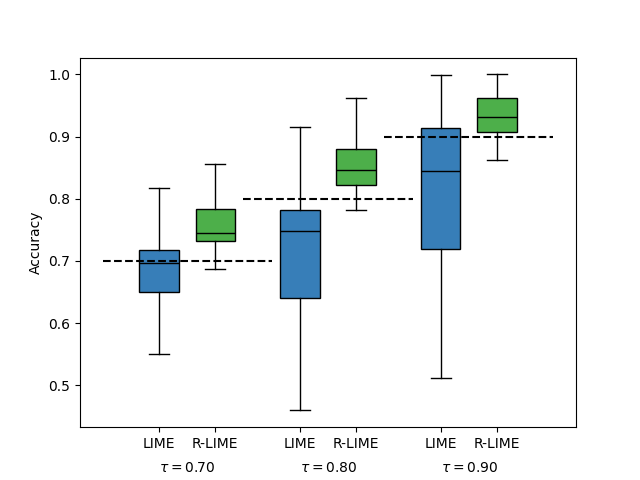
\includegraphics[width=0.55\textwidth]{python/exp2/box_plot}
  \caption[Comparison of Local Accuracy between R-LIME and LIME]{%
    Comparison of local accuracy between LIME and R-LIME.
    We generated explanations for 100 instances using each method
    and calculated the accuracy for each method within the 10,000 instances
    sampled inside the rectangular region obtained by R-LIME.
  }\label{fig:box_plot}
\end{figure}
The results are presented in \cref{fig:box_plot}, showcasing the distribution of the accuracy of the linear approximation models obtained by LIME and R-LIME.
R-LIME exhibits higher accuracy compared to LIME for all values of $\tau$. This suggests that the linear approximation models learned by LIME and R-LIME differ significantly, and R-LIME learns a high-precision linear approximation model adapted to the rectangular region. Additionally, as $\tau$ increases, the variability in the accuracy of LIME widens. This indicates that the linear models learned by LIME may not function effectively as approximation models depending on how the region is selected.

\section{Challenges and Future Perspectives}
 
 {%
  \def\imgwidth{0.49\textwidth}
  \begin{figure}[t]
    \centering
    \begin{subfigure}[t]{\imgwidth}
      \centering
      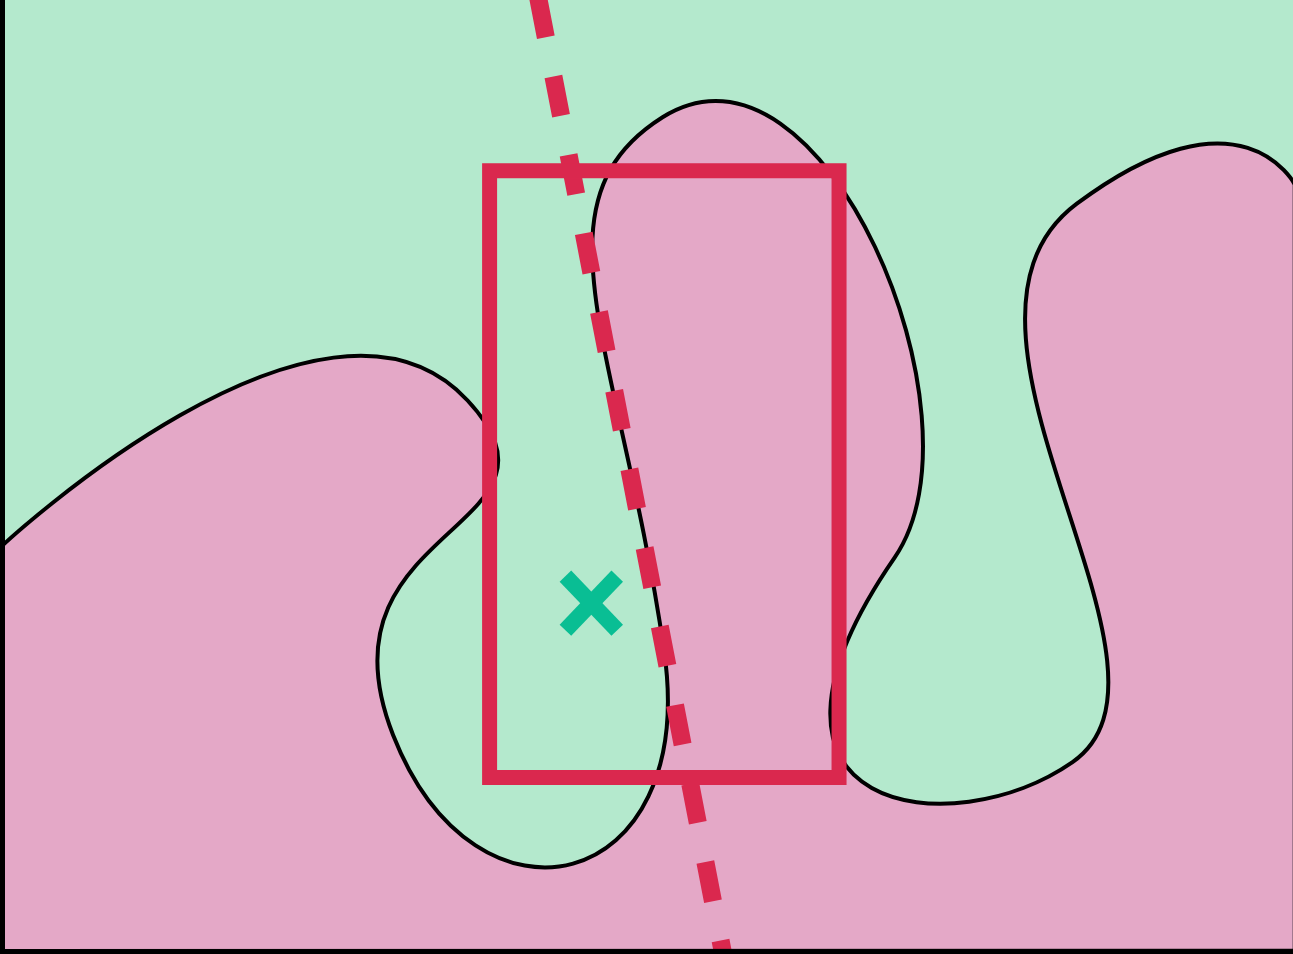
\includegraphics[width=0.78\textwidth]{newlime}
      \caption{R-LIME for balanced data.}\label{fig:balanced}
    \end{subfigure}
    \begin{subfigure}[t]{\imgwidth}
      \centering
      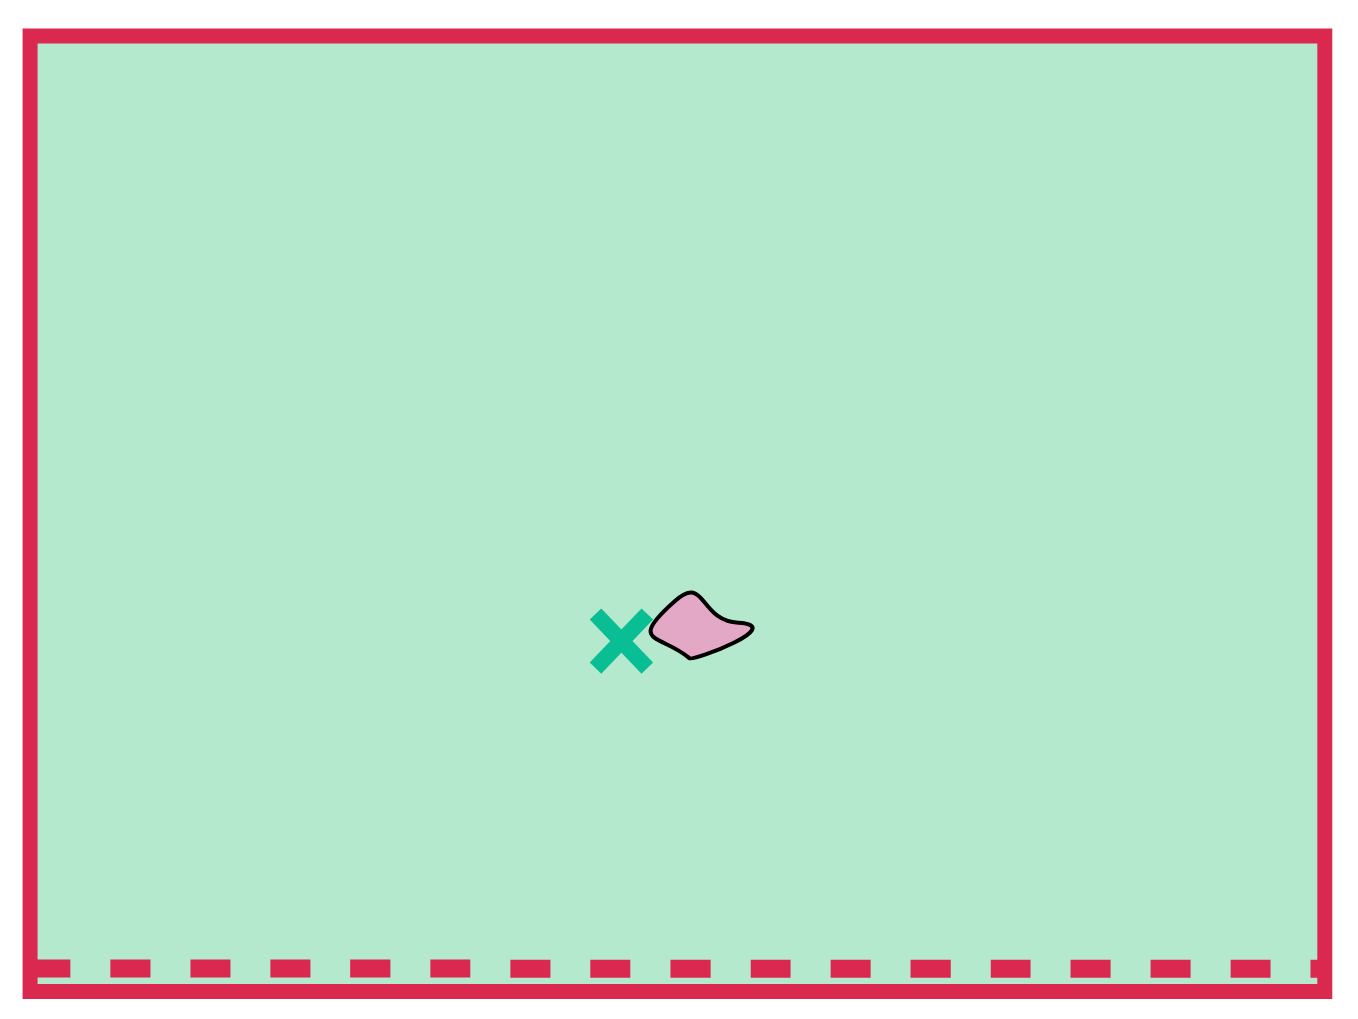
\includegraphics[width=0.8\textwidth]{newlime_for_imbalanced_data}
      \caption{R-LIME for imbalanced data.
      }\label{fig:imbalanced}
    \end{subfigure}
    \caption{%
      Behavior of R-LIME for balanced and imbalanced data.
      In case of imbalanced label distribution, 
      the approximation region covers the entire input space and the
      linear approximation model always outputs the majority label.
    }
    \vspace{10pt}
  \end{figure}
 }

\subsection{Behavior Regarding Imbalanced Label Distribution}
R-LIME may generate less useful explanations when there is bias in the distribution of black-box model outputs. When the distribution of black-box model outputs is significantly biased for a given accuracy threshold $\tau$ (the ratio of the majority label is less than $\tau$), the approximation region generated by R-LIME covers the entire input space, and the learned linear approximation model always outputs the majority label (\cref{fig:imbalanced}).

As a first solution to this problem, changing the loss function is considered. Using weighted logistic loss or Focal Loss \cite{lin2020focal} as the loss function might lead to the generation of more useful explanations in the case of imbalanced label distribution. Another solution involves adding constraints to limit the label distribution bias within the approximation region. In addition to \cref{eq:const_prec}, adding a constraint like
\begin{equation}
  {\left(\mathbb{E}_{z\sim\mathcal{D}(z\mid A)}[\mathbbm{1}_{f(z)=1}]-\frac{1}{2}\right)}^2<\mu
\end{equation}
could suppress the excessive expansion of the approximation region.

\subsection{Changes in Reward Distribution in Optimal Arm Identification}\label{sec:reward}
{%
  \renewcommand{\arraystretch}{1.1}
  \begin{table}[tbp]
    \centering
    \caption{%
      Deviation between the estimated accuracy and the true accuracy.
    }\label{tab:reward}
    \begin{tabular}{cccc}
  \toprule
                     & Estimated acc. & True acc. & Deviation \\
  \midrule
  Average            & .811           & .829      & .012      \\
  Standard Deviation & .018           & .023      & .017      \\
  \bottomrule
\end{tabular}

  \end{table}
}
In R-LIME, the problem of selecting the rule with the highest accuracy is formulated as the optimal arm identification problem in multi-armed bandit theory, solved using the KL-LUCB algorithm \cite{kaufmann2013information}. However, this algorithm assumes that the reward distribution remains constant, while in R-LIME, the reward distribution (accuracy of the linear approximation model) changes with every update of the approximation model after sampling. Therefore, rewards obtained at an early stage when the accuracy is still low might influence the estimated value and deviate from the true value.

An experiment was conducted to evaluate the deviation between the estimated accuracy and the true accuracy. Explanations were generated for 3,200 data instances sampled from the dataset, and the estimated accuracy was compared with the true accuracy. The true accuracy was calculated based on 1,000 instances sampled within the approximation region, considering cases where the outputs of the black-box model and the linear approximation model matched. The results in \cref{tab:reward} show a mean deviation of 0.012 with a standard deviation of 0.017. While the deviation is relatively small, improvements to the selection algorithm need to consider the changing accuracy.

\subsection{Evaluation through User Studies}
Given the nature of the field of "interpretable machine learning,"
where the goal is to "interpret" machine learning models,
it is challenging to quantitatively compare various methods.
While quantitative experiments were conducted in \cref{sec:exp2},
they mainly demonstrated that the proposed method generates
locally accurate explanations compared to LIME.
The results do not directly prove the high interpretability of the proposed method.

One potential method to quantitatively evaluate "interpretability" is through user studies. For example, \cite{ribeiro2018anchors} conducted user studies, assuming that if users could predict the output of a black-box model with high accuracy based on provided explanations, those explanations contained valuable information about the model's behavior. Similarly, conducting user studies in this research would be desirable to evaluate the interpretability of the proposed method.

\section{Conclusion}
We identified challenges in existing methods for local model-agnostic post-hoc
explanations of black-box classifiers and proposed R-LIME to address them.
We represented the rectangular region for local linear approximation as a
conjunction of predicates of features and proposed an algorithm to
maximize coverage under the constraint of minimum approximation accuracy.
Comparing the outputs of LIME and R-LIME on real-world datasets,
we demonstrated that explanations provided by R-LIME have clearer application
scopes and can be evaluated by users for reliability and generality.
However, we discussed the instability of behavior concerning imbalanced label
distributions and raised questions about the theoretical validity of using
the KL-LUCB algorithm.

% \subsection{A Subsection Sample}
% Please note that the first paragraph of a section or subsection is
% not indented. The first paragraph that follows a table, figure,
% equation etc.\ does not need an indent, either.
%
% Subsequent paragraphs, however, are indented.
%
% \subsubsection{Sample Heading (Third Level)} Only two levels of
% headings should be numbered. Lower level headings remain unnumbered;
% they are formatted as run-in headings.
%
% \paragraph{Sample Heading (Fourth Level)}
% The contribution should contain no more than four levels of
% headings. Table~\ref{tab1} gives a summary of all heading levels.
%
% \begin{table}
% \caption{Table captions should be placed above the
% tables.}\label{tab1}
% \begin{tabular}{|l|l|l|}
% \hline
% Heading level &  Example & Font size and style\\
% \hline
% Title (centered) &  {\Large\bfseries Lecture Notes} & 14 point, bold\\
% 1st-level heading &  {\large\bfseries 1 Introduction} & 12 point, bold\\
% 2nd-level heading & {\bfseries 2.1 Printing Area} & 10 point, bold\\
% 3rd-level heading & {\bfseries Run-in Heading in Bold.} Text follows & 10 point, bold\\
% 4th-level heading & {\itshape Lowest Level Heading.} Text follows & 10 point, italic\\
% \hline
% \end{tabular}
% \end{table}
%
%
% \noindent Displayed equations are centered and set on a separate
% line.
% \begin{equation}
% x + y = z
% \end{equation}
% Please try to avoid rasterized images for line-art diagrams and
% schemas. Whenever possible, use vector graphics instead (see
% Fig.~\ref{fig1}).
%
% \begin{figure}
% 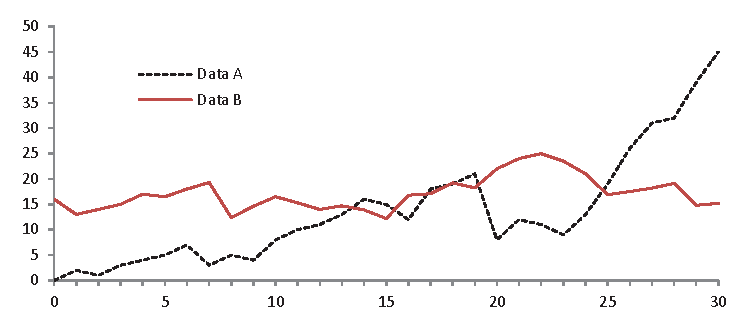
\includegraphics[width=\textwidth]{fig1.eps}
% \caption{A figure caption is always placed below the illustration.
% Please note that short captions are centered, while long ones are
% justified by the macro package automatically.} \label{fig1}
% \end{figure}
%
% \begin{theorem}
% This is a sample theorem. The run-in heading is set in bold, while
% the following text appears in italics. Definitions, lemmas,
% propositions, and corollaries are styled the same way.
% \end{theorem}
% %
% % the environments 'definition', 'lemma', 'proposition', 'corollary',
% % 'remark', and 'example' are defined in the LLNCS documentclass as well.
% %
% \begin{proof}
% Proofs, examples, and remarks have the initial word in italics,
% while the following text appears in normal font.
% \end{proof}
% For citations of references, we prefer the use of square brackets
% and consecutive numbers. Citations using labels or the author/year
% convention are also acceptable. The following bibliography provides
% a sample reference list with entries for journal
% articles~\cite{ref_article1}, an LNCS chapter~\cite{ref_lncs1}, a
% book~\cite{ref_book1}, proceedings without editors~\cite{ref_proc1},
% and a homepage~\cite{ref_url1}. Multiple citations are grouped
% \cite{ref_article1,ref_lncs1,ref_book1},
% \cite{ref_article1,ref_book1,ref_proc1,ref_url1}.

\subsubsection{Acknowledgements}
% Please place your acknowledgments at
% the end of the paper, preceded by an unnumbered run-in heading (i.e.
% 3rd-level heading).
I would like to express my gratitude to Associate Professor Keigo Kimura from the Department of Mathematical Science, Division of Information Recognition, Graduate School of Information Science and Technology, Hokkaido University. He provided invaluable guidance, from setting the research theme to outlining the strategy and content of this study. Additionally, I appreciate the diverse insights shared by Professor Mineichi Kudo in the same laboratory. Finally, I am deeply thankful to all the members of the laboratory for their helpful advice and collaboration throughout the research process.

%
% ---- Bibliography ----
%
% BibTeX users should specify bibliography style 'splncs04'.
% References will then be sorted and formatted in the correct style.
%
\bibliographystyle{splncs04}
\bibliography{MyRef/ref}
%
\end{document}
